\chapter{Experimental Methods}
The main goal of the experiment is to determine the \be-\al\ angular correlation. The experiment was done at the IGISOL facility, at the University of Jyväskylä \cite{igisol}. The experiment took place in august 2020, delayed by the ongoing corona pandemic. This chapter will be concerning the experimental setup, a discussion of the detectors and an overview of the software used to extract and analyze the data. 


\section{Experimental setup}
The setup is designed mainly for the decay of \isotope[12]{B} measured in the same experiment. In that decay three-alpha particles are emitted in less than 1\% of the decays and the setup should therefore have a high efficiency and be able to measure \al-particles in an environment with many beta-particles. \\

The setup is able to measure \be-\al\ angular correlations in the $\beta$-delayed particle decay of \isotope[8][]{Li}. When measuring multiple particles, the setup is highly dependent on the coverage of the solid angle. Therefore the setup is designed to have a large solid angle coverage, with high $\alpha$-particle resolution, while still being able to measure $\beta$-particles.\\
This is has been achieved by creating a cube of six double sided silicon detectors (DSSD), all backed by a unsegmented silicon detectors (PAD). To attain the largest solid angle, the detectors where placed as close to one another as possible. A 3D printed case was designed to hold the detectors in place, and achieved a solid angle coverage of 51\% for the DSSD's, which can be seen on \cref{fig:cubepic}. An illustration of the setup, together with the different detectors' thickness can be seen on \cref{fig:opstilling}. 
Even though the setup was designed to hold 12 detectors in total, there where only 11 detectors in the actual experiment. The PAD behind Det1 was defect, and was therefore removed. 

\begin{table}[H]
	\centering
	\begin{tabular}{ll|ll}
		Detector & Thickness {[}$\mu$m{]} & PAD & Thickness{[}$\mu$m{]} \\ \hline
		Det1     & 67                     & n/a & n/a                   \\
		Det2     & 1002                   & P2  & 1036                  \\
		Det3     & 65                     & P3  & 1497                  \\
		Det4     & 60                     & P4  & 1490                  \\
		DetU     & 60                     & PU  & 1498                  \\
		DetD     & 1043                   & PD  & 1038                 
	\end{tabular}
\end{table}

\begin{figure}[h]
	\centering
	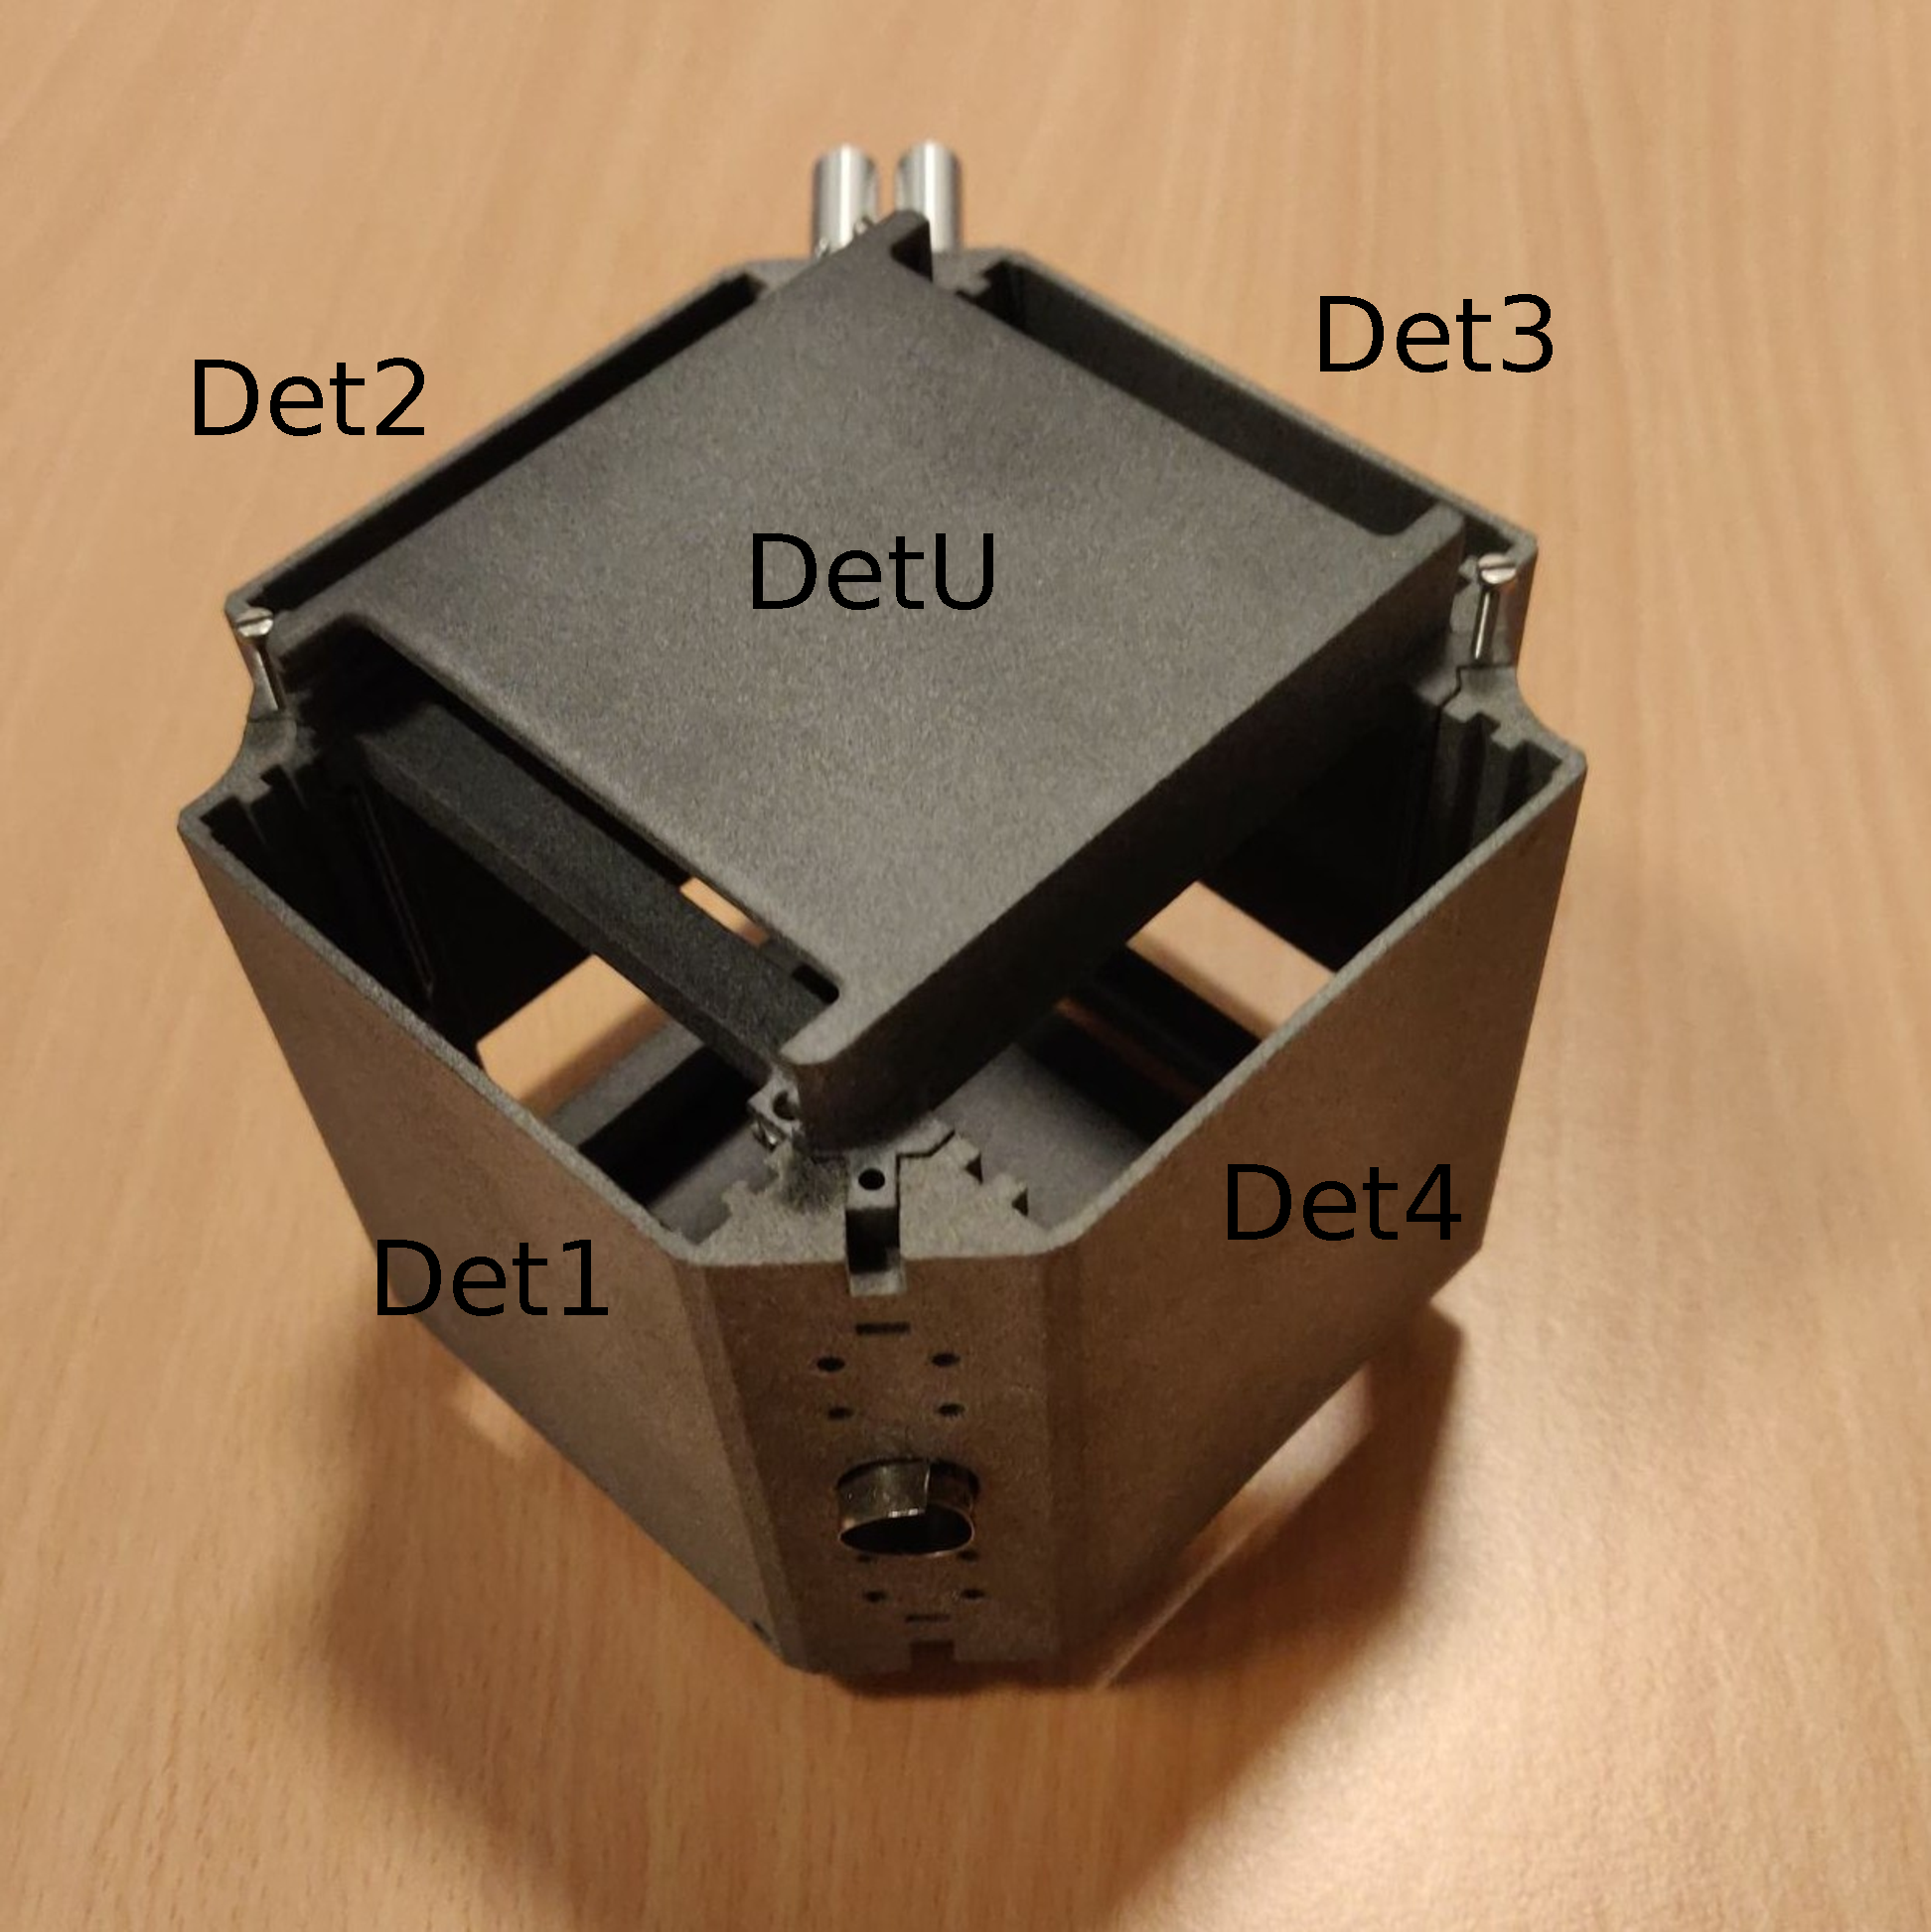
\includegraphics[width=.6\linewidth]{../figures/cubepic.pdf}
	\caption{A picture of the 3D printed cube used to hold all detectors in place. The placement of the detectors have been shown, with exception of DetD, which was at the bottom of the cube. The beam enters through the metal ring between Det1 and Det4}
	\label{fig:cubepic}
\end{figure}

\begin{figure}[H]
	\centering
	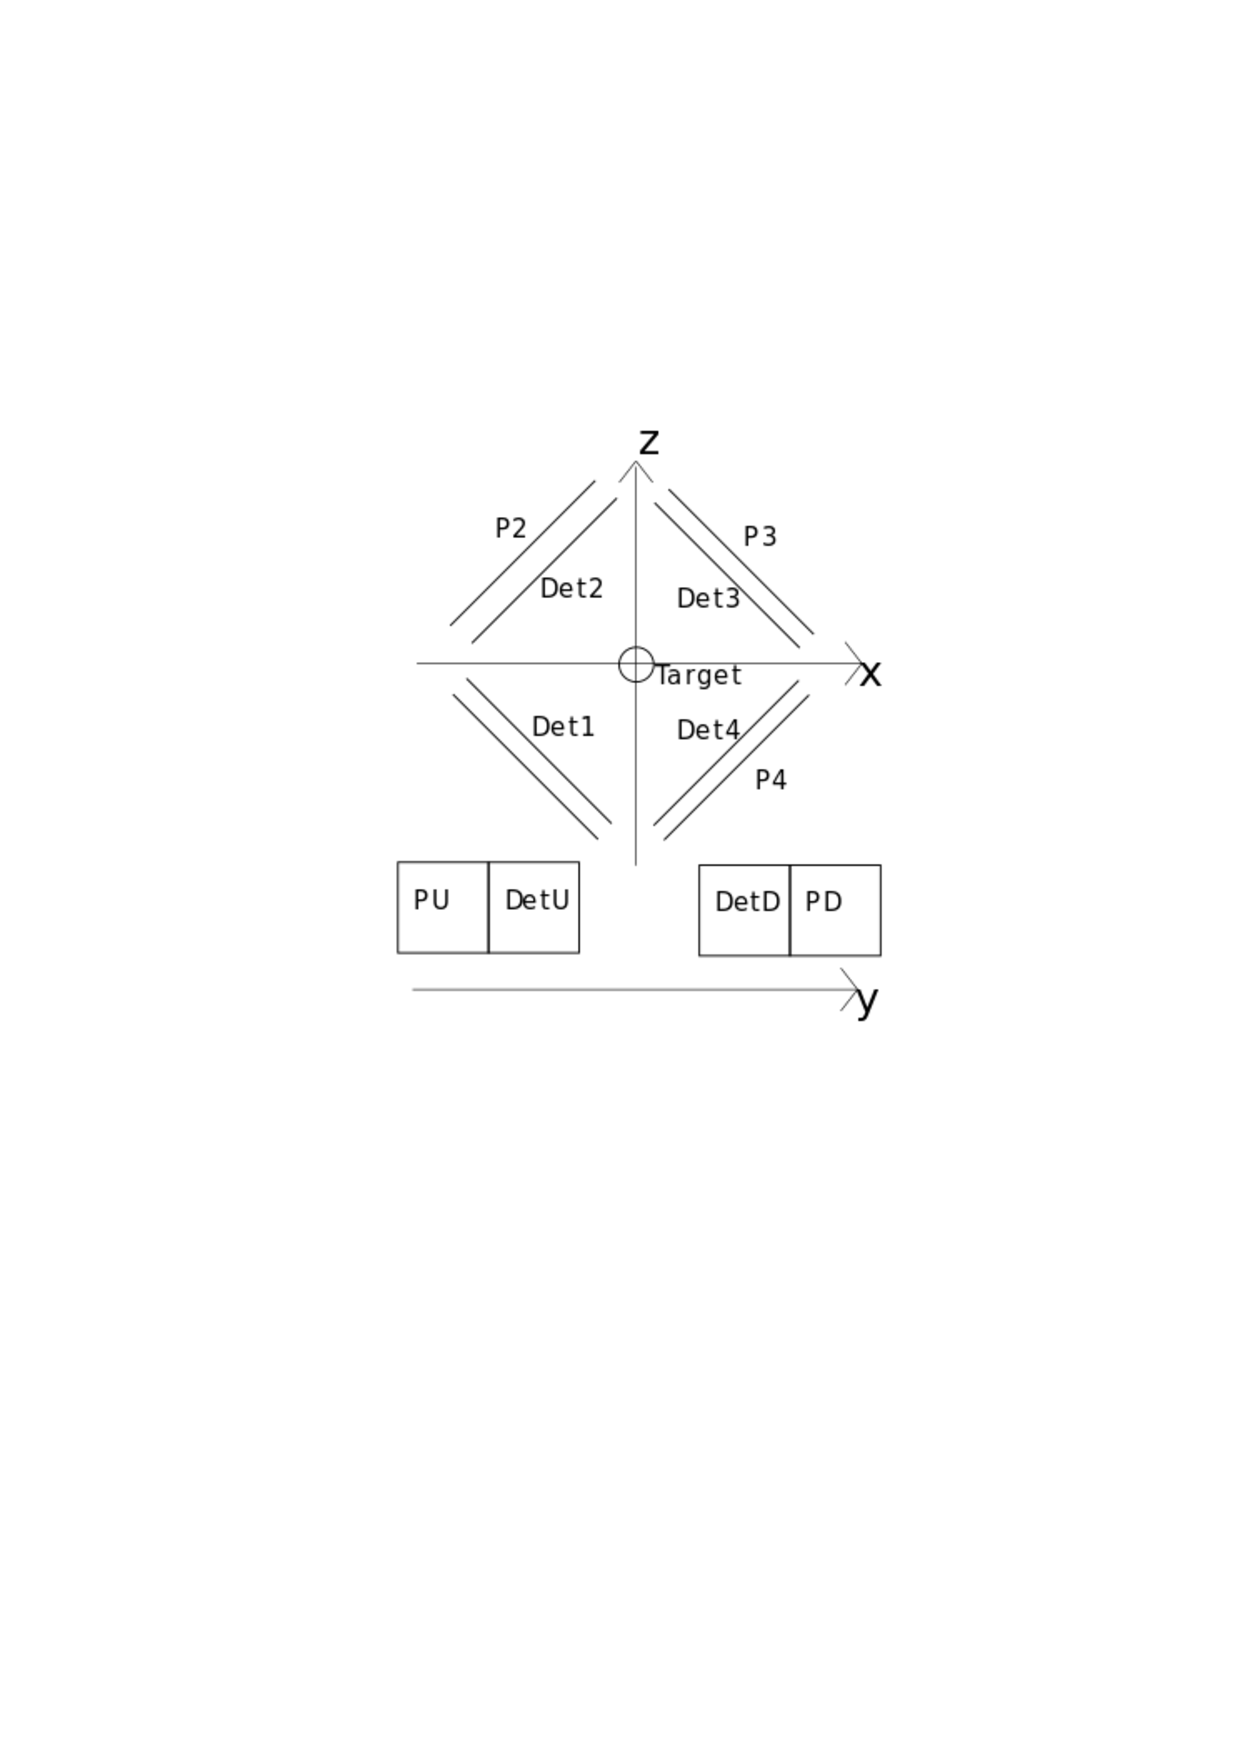
\includegraphics[width=.6\linewidth]{../figures/opstilling_better.pdf}
	\caption{An illustration of the setup. Det1-Det4 are placed around the target, facing the target which is located at the center of the coordinate system. DetU is above the target, and DetD is below the target. Behind each detector is a PAD, with the exception of Det1, who's PAD was defect. The beam is parallel to the z-axis, entering the setup from the negative z-direction.}
	\label{fig:opstilling}
\end{figure}

\section{The detectors}
As mentioned above, there where two types of detectors present in the setup. The first type is the Double sided silicon detector. 
As the name suggests, it consists of two sides, a front layer and a back layer. Each layer consists of 16 strips, that are placed in rows next to each other. The two layers are then arranged so each side are mutually orthogonal, which effectively makes pixels where each strip intersects a strip on the other side \cite{TENGBLAD2004458}. An illustration of the detector can be seen on \cref{fig:W1}.\\
The strips on the front side are p-doped, while the back side are n-doped. When a charged particle hits the detector, it will ionize the atoms in the semi-conductor, and produce a electron-hole pair. The number of electron-hole pairs is proportional to the energy of the charged particle. 
The bias voltage on the detector collects the electrons and holes on opposite sites of the strip, where the charge is collected on aluminum contacts and a signal is measured. Energy is not deposited in these contacts, and therefore they constitute to a so called dead layer. \\
The detectors are square $5\times 5$ \SI{}{cm} and with their $16\times 16$ strips, they have an effective gird of  256 pixels of \SI{9}{mm}. 
4 of the 6 detectors have a thickness of \SI{60}{\mu m} and a \SI{100}{nm} dead layer. These  are Det1, Det3, Det4 and DetU in the setup seen on \cref{fig:opstilling}. The other 2 detectors (Det2 and DetD) are both \SI{1000}{\mu m}.
\\
\\
The other type of detector is the PAD. They are different from the DSSD's, in that they do not have sides, and no strips. Therefore they do not contain a grid, the same way the DSSD's do, and will not provide any information as to where a particle has hit. But they are included in the setup to detect excess energy of particles not stopped by the DSSD. This makes them good at detecting \be-particles, as they will not be stopped by a DSSD.

\begin{figure}[h]
	\centering
	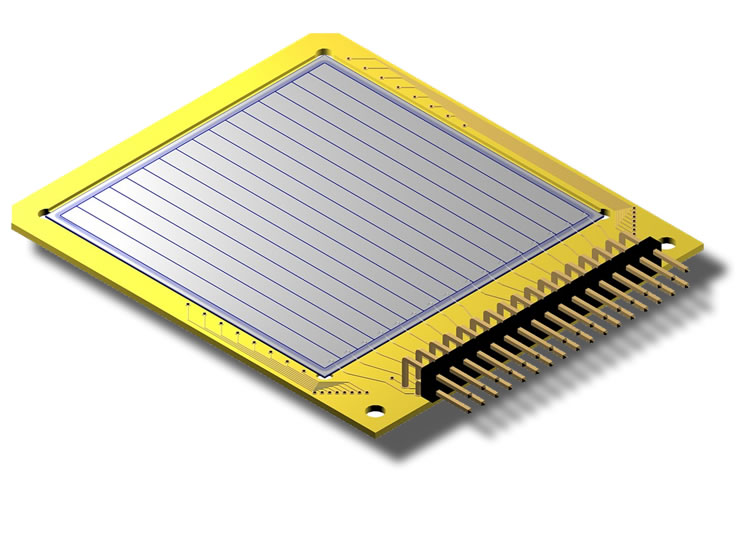
\includegraphics[width=\columnwidth]{../figures/W1.jpg}
	\caption{An illustration of the DSSD type used in this experiment. The detector has 16 p-doped strips, and 16 n-doped strips perpendicular on the other side. This gives 256 pixels on the detector in total. Image courtesy of Micron Semiconductor Ltd \cite{detector}.}
	\label{fig:W1}
\end{figure}

An $\alpha$-particle will deposit all of its energy into the first DSSD it encounters, and be effectively stopped completely by it, and a $\beta$-particle will deposit almost no energy in a thin DSSD, and travel through it, ending up depositing some energy in the PAD. \\
Therefore one can roughly distinguish the $\alpha$-particles from the $\beta$-particles, by observing whether a particle has hit the DSSD and the PAD. \\
\\
Since there are also two thick DSSD's in the setup, one can also get some information from a $\beta$-particle from these thicker detectors, as it will deposit more energy in these detectors. 




\section{AUSAlib and ROOT}
ROOT \cite{ROOT} is an object oriented C++ framework that is designed primarily for data analysis in high-energy and nuclear physics. It was created at CERN in 1995, and has since grown and become the dominant analysis software at both CERN and many other nuclear and particle physics laboratories. 
ROOT was designed to handle large amounts of data with high computing efficiency. \\
ROOT makes an intelligent data structure by creating a "Tree" with the class \texttt{TTree}. This tree will then have "branches" which corresponds to some variable of the given detection event, such as the energy of the front strip or identity of the detector. This \texttt{TTree} then allows for reading of an individual branch, while ROOT takes care of the memory management. One can also store a \texttt{TTree} to the disk in the form a .root file. \\

ASUALib \cite{AUSA} is a tool that build on top of ROOT. It was created by the subatomic group at Aarhus University.
Before this tool was created, everyone in the group had to more or less create their own tools to get data from the detectors into a useful data structure. This meant that a lot of time was wasted just trying to access data from experiments. AUSAlib was therefore created, so the basic tasks of data extraction was automated. \\
AUSAlib has a lot of functionalities, but the two main tools that was used to extract data was the \textit{Sorter} and \textit{Calibrator}.

\subsection{Unpacker}
The \texttt{Unpacker} converts raw data from the detectors into a ROOT \texttt{TTree}. This is done by using the unpacking program \texttt{ucesb} \cite{ucesb}. This will setup the branch structure of the data. Some of these branches are \texttt{FT} and \texttt{BT}, which is a vector of the time (\texttt{TDC}) values for each event, for the front and backside of the detector. They are vectors because they contain information for each particle hits in a given time slot, for which there can be multiple. 
There are also the branches \texttt{FE} and \texttt{BE}, which is the energy (\texttt{ADC}) (energy) associated with the events. 

\subsection{Calibrator}
Since the detectors work, by measuring an electrical charge that comes from the charged particle, the detectors needs to translate a specific charge to energy deposited. \\
To do that, we use the \texttt{Calibrator}-tool, which is designed to convert a channel number into an actual energy. Assuming that the channel numbers are linearly related to the energies, a known radioactive source can be measured, and the expected spectrum can be compared to the measured. This is done for each strip in each detector.
\\
\\
The \texttt{Calibrator} starts by running a peak-finding algorithm over some calibration data, to roughly identify the locations of the peaks, followed by a multi-Gaussian fit to find the most precise peak location. 
The positions of the peaks can then be compared to the expected energies, giving an associated energy to a given channel. \\
\\
As mentioned earlier, all of the detectors have a small aluminum dead layer. All particles that pass through this layer will loses some amount of energy depending on the stopping power of the material and the effective thickness of the dead layer $\Delta x_{eff}$, which furthermore depends on the angle of incidence, $\theta$. 
The relationship between the effective thickness and the actual thickness is described as $\Delta x_{eff} = \Delta x/ \cos(\theta)$. This gives the measured energy as 
\begin{equation*}
E' = E - \dfrac{dE}{dx} \dfrac{\Delta x}{\cos(\theta)},
\end{equation*}
where $E$ is the original energy of the particle, $dE/dx$ is the stopping power of the material and $\Delta x$ is the thickness of the dead layer. The stopping power is calculated from SRIM \cite{ZIEGLER20101818} \\
\\
These calculations are all handled by the \texttt{Calibrator}. 
As input it takes an unpacked measurement of a source, a file specifying the locations of the expected peaks and a file specifying the spacial locations of the detectors. 
From this it calculates the energy loss, and creates a linear relationship between channel numbers and energies. This is then written to the disk as a seperate calibration file, which can be parsed to other modules.\\
It is important to note that the Calibrator does not modify any data. Therefore the energy loss is unaccounted for. Instead it corrects the expected energy spectrum, which means that the resulting calibration is still valid. The energy loss correction is therefore still needed in the analysis, as the effect is unaccounted for in measurements. 


\subsection{Sorter}
The sorter is used after a successful calibration. It generates a ROOT file based on the unpacked data, and applies the calibration. 
It is also responsible for matching and combining events from the front-side to the back-side of the detector. If there where one hit in the front side and one in the back, the mathcing is fairly trivial. If there however where multiple hits in both front and back, the \texttt{Sorter} will run a matching algorithm, which pairs the hits with the lowest energy differences. \\
\\
When the events have been matched, the hits on the individual sides of each detector are merged into a single event. 
Therefore each event can now be considered a multiple of particle hits. This makes it possible to associate physical properties with each particle, such as direction and energy. 
There has still not been done any filtering of the data, which is what we will discuss in  \cref{cha:dataReduction}.


